\documentclass{scrartcl}
% Comment the following line to NOT allow the usage of umlauts
\usepackage[utf8]{inputenc}
\usepackage[spanish]{babel}
\selectlanguage{spanish}
\usepackage{xcolor}
\usepackage{tcolorbox} %para cajas de texto
\usepackage{sectsty}
\usepackage{hyperref}
%\usepackage{color}
\usepackage{bbding}
\definecolor{hd}{rgb}{0.2,0.2,0.7}
\definecolor{tit}{rgb}{0.1,0.4,0.7}
\usepackage{amssymb}
% Fifure in italics

\usepackage[format=plain,
labelfont=it]{caption}

\sectionfont{\color{hd}} 
\subsectionfont{\color{hd}} 
\subsubsectionfont{\color{hd}} 

% save figure on top
\makeatletter
\setlength{\@fptop}{0pt}
\makeatother

\graphicspath{{../figs/}}

% Uncomment the following line to allow the usage of graphics (.png, .jpg)
%\usepackage{graphicx}
\title{\color{tit} Doing bayesian data analysis\\
		by Kruschke}
	\subtitle{Revisión} 
\author{\normalsize J. E. Alcalá \\
		\normalsize CEIC, Universidad de Guadalajara} 
\date{\today} 
% Start the document
\begin{document}
\maketitle 
	\section{Capítulo 4: What is this stuff called probability?}
	\subsection{Preliminares}
	
	\begin{tcolorbox}[title=Definiciones]
		\textbf{Variable aleatoria}: es una función que mapea los resultados de un experimento aleatorio al conjunto de los números reales (comúnmente). Se suele representar con letra mayúscula (e.g., $X$).\\
		\textbf{Espacio muestral}: el conjunto de todos los resultados posibles. Se suele representar con $\Omega$. De este conjunto la $X$ mapea a los reales: $X: \Omega \rightarrow \mathbb{R}$. Es decir, a cada elemento de $\Omega$ asigna un número real, $X(\omega)$.\\
		\textbf{Evento}: subconjunto de $\Omega$, usualmente representado por una vocal mayúscula, e.g., $A$. Si lanzamos una moneda dos veces, $\Omega = \{HH,HT,TT,TH\}$. El evento ``la primera moneda cae H'' es $A=\{HH,HT\}$. \\
		\textbf{Probabilidad}: la función $p(A)$ asigna un valor numérico a cada evento $A$. Se llama probabilidad de $A$ si satisface los siguientes axiomas:
		\begin{itemize}
			\item \textbf{Axioma 1:} $p(A) \geq 0$ para cada $A$. Es decir, $p(A)$ es positiva.
			\item \textbf{Axioma 2:} $p(\Omega) = 1$.
			\item \textbf{Axioma 3:} para los eventos $A_i,A_j..., i \neq j$ (es decir, si son disjuntos), 
			\[p\Bigg (\bigcup^\infty_{i=1} A_i \Bigg) = \sum_{i=1}^{\infty} p(A_i)\]
		\end{itemize}
		
	\end{tcolorbox}

	\begin{figure}[t!]
		\centering
		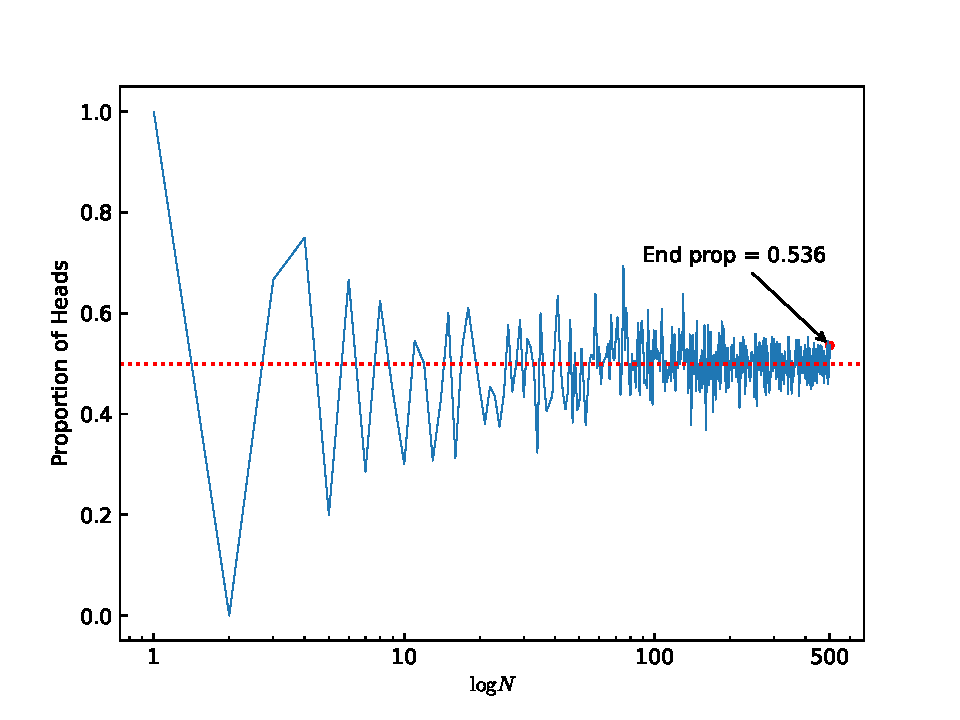
\includegraphics[width=0.8\textwidth]{Figure_2.pdf}
		\caption{Proporción de $H$ al lanzar una moneda $1,2,..,N$. La proporción se calcula con $\sum_{i=1}^{N}\mathbb{I}_{\omega = H}\times (1/i)$. Conforme $i = N,N \rightarrow \infty $, la proporción de $H \rightarrow p(H)$}
		\label{fig:fig2}
	\end{figure}
	
\end{document}